% !TEX root = ../00_thesis.tex
%-------------------------------------------------------------------------------
\section{Designing \triscale}
\label{sec:triscale}
%-------------------------------------------------------------------------------

In this section, we first describe the data analysis performed by \triscale and how the analysis procedure is linked to the design of experiments~(\cref{subsec:metrics} to \cref{subsec:repeatability}).
We then illustrate how the formalism introduced by \triscale allows to unambiguously describe an entire performance evaluation with only a handful of parameters~(\cref{subsec:parameters}).
Thereafter, we detail the robust and non-parametric statistical methods used by \triscale~(\cref{subsec:triscale_stats}), and discuss how the framework assists a user in deciding the required time span for a series of runs~(\cref{subsec:network_profiling}).
We finally show how \triscale helps assessing the reproducibility of experiments by computing a variability score~(\cref{subsec:reproducibility}).

%-------------------------------------------------------------------------------
\subsection{Runs and Metrics}
\label{subsec:metrics}

\afterpage{
\begin{figure}
    \centering
    \begin{subfigure}{\linewidth}
        \centering
       	\href{\triscalefig{Figure-3a}}{
        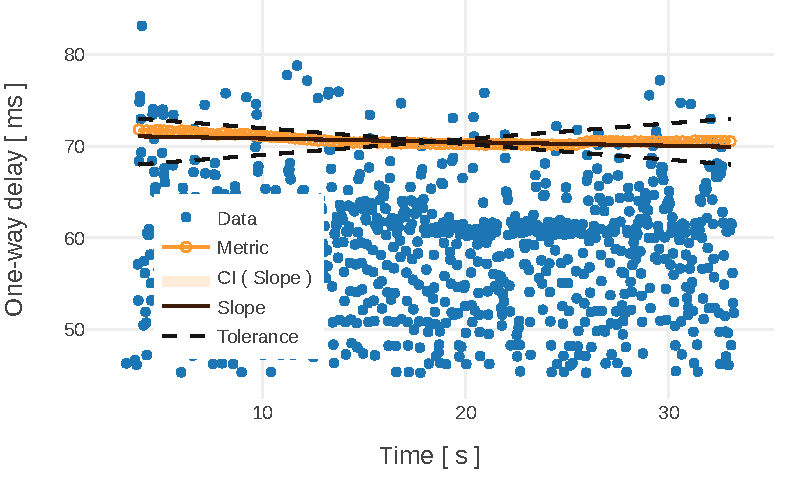
\includegraphics[scale=1]{Figures/plot_example_metric.pdf}}
        \caption{\raggedright Raw data (one-way delay) and metric data (95th percentile).}
        \label{fig:analysis_metric}
    \end{subfigure}



    \begin{subfigure}{0.45\linewidth}
        \centering
       	\href{\triscalefig{Figure-3b}}{
        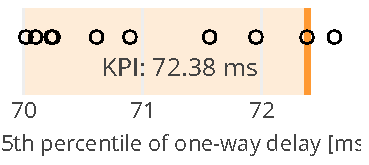
\includegraphics[scale=1]{Figures/plot_example_KPI.pdf}}
        \caption{Runs' metric data and corresponding KPI value.}
        \label{fig:analysis_kpi}
    \end{subfigure}
    %
    \hfill
    \begin{subfigure}{0.45\linewidth}
        \centering
     	  \href{\triscalefig{Figure-3c}}{
        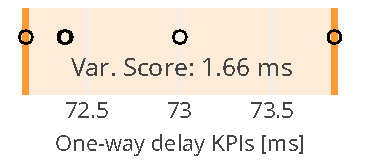
\includegraphics[scale=1]{Figures/plot_example_var_score.pdf}}
        \caption{Series' KPI data and corresponding variability score.}
        \label{fig:analysis_score}
    \end{subfigure}
    \caption{Example plots produced by \triscale during the data analysis.
    \Cref{fig:analysis_metric}: computation of the metric (95th percentile on one-way delay) with convergence test (confidence 95\%, tolerance 1\%).
    \Cref{fig:analysis_kpi}: computation of the KPI (75th percentile with 75\% confidence).
    \Cref{fig:analysis_score}: computation of the variability score (25-75th percentiles with 75\% confidence).
    \capt{Sample data from the case study (\cref{sec:triscale_eval}) for the \textit{FillP} congestion-control scheme.}}
    \label{fig:analysis_examples}
\end{figure}
}

A \triscale's metric evaluates a performance dimension across one run. For example, a metric may be the average throughput achieved by a congestion-control scheme over 30\s runtime of a full-throttle flow.
Computing a metric takes the following inputs.

\fakepar{Inputs}
\custommini),  &\\
          & tolerance & $t$   &(\textit{default: 1\%})    &\}
    \end{tabular}
  \item The raw data of the run.
  \end{itemize}
}%


In its current implementation, \triscale supports only percentiles as measures.
This can be easily extended to offer a catalog of common measures for networking experiments~(mean, max, fairness index, \etc).

\fakepar{Procedure}
If the run is expected to convergence, \triscale starts by performing a convergence test.
The purpose of the convergence test is to assess whether the metric measure has reached a ``stable'' value by the end of the run, and therefore if it is a good estimate of the ``long-running'' performance.

To test this, \triscale divides the raw data in 200 chunks. First, it considers the first 100 chunks (\ie the first half of the data) and computes a first value of the measure. Then, \triscale adds one chunk of data and recomputes a new measure value (\ie using the first 101 chunks). The process repeats until all chunks are used, leading to a set of 100 measure values. \triscale performs its convergence test~(detailed in \cref{subsec:triscale_stats}) on the measure data.
This procedure (i)~tests what we are interested in (\ie the convergence of the \emph{measure}, not of the protocol in general) and (ii)~smooths the effects of ramp-up time by computing the first measure with already half of the run data.
If the test is passed, \triscale returns the median of the measure data as the metric measure for the run.

\begin{remark}
  The choice of 200 chunks is arbitrary. We choose this value as it is practical and leads to 100 measure data samples. Empirically, we found this is enough to reliably test for the metric convergence.
\end{remark}

\begin{remark}
  If there are less than 200 raw data points, \triscale reduces the number of chunks to the number of data points.
  \triscale (arbitrarily) sets a minimum of 20 data points for a convergence test.
\end{remark}

\fakepar{Outputs}
\custommini{%
\begin{itemize}
  \item
  The result of the convergence test (if performed),
  \item
  The metric value for the run,
  \item
  Textual logs; plot of the input data and metric (\Cref{fig:analysis_metric}).

\end{itemize}
}

\fakepar{Link to the experiment design}
The computation of \triscale metrics is linked to the definition of the \emph{runtime}; \ie how long a run should be.
If the evaluation scenario is terminating (\eg transmit 1\MB through a link), the runtime must be long enough to complete the task.
If the evaluation is ``long-running'' (\eg one-way delay in a full-throttle flow), the runtime must be long enough for the metric (the one-way delay) to converge (convergence test details in \cref{subsec:triscale_stats}).
\triscale can analyze preliminary experiments to estimate the required runtime: by performing increasing long runs and test for convergence~(illustrated in \cref{sec:triscale_eval}).

%-------------------------------------------------------------------------------
\subsection{Series and KPIs}
\label{subsec:KPIs}
%-------------------------------------------------------------------------------

\triscale's key performance indicators (KPIs) evaluate performance dimensions across a series of runs.
Performing multiple runs allows to mitigate the inherent variability of the experimental conditions.
KPIs capture this variability by estimating percentiles of the (unknown) metric distributions.
Concretely, a \triscale KPI is a one-sided CI of one percentile; \eg a lower-bound for the 75th percentile of the delay metric estimated with a 75\% confidence level.
Computing a KPI takes the following inputs.

\fakepar{Inputs}
\custommini{%
  \begin{itemize}
    \item
    The {KPI} definition\\
    \begin{tabular}{@{\quad}l@{\quad}r@{\;\;:\;\;}l@{\quad}l}
      \{  & percentile & $p$ &\\
          & confidence & $C$&\}
    \end{tabular}
    \item
    The metric data (computed from a series of runs).
\end{itemize}}


\fakepar{Procedure}
To compute the KPI (\ie to compute a CI for a given percentile), \triscale uses the Thompson's method (\cref{subsec:triscale_stats}), which requires the input data to be \iid.
Thus, \triscale starts by performing an independence test~(\cref{subsec:triscale_stats})
on the metric data before computing the KPI.

\fakepar{Outputs}
\custommini{
\begin{itemize}
  \item The result of the independence test,
  \item The KPI value for the series of runs,
  \item Textual logs; plot of the metric data and corresponding KPI (\Cref{fig:analysis_kpi}).
\end{itemize}
}

\fakepar{Link to the experiment design}
The computation of \triscale KPIs is linked to the definition of the number of runs in a series (\emph{\#\,runs}) and the series time span (\emph{span}).
The minimal number of runs in a series directly follows from the definition of the KPI; \ie the percentile to estimate $p$ and the desired confidence level $C$.
The series time span refers to the time interval used for scheduling the runs in a series (\ie when to run the experiment).
This is important because networks often feature time-dependent conditions; for example, there may be systematically more cross-traffic during daytime than nighttime. Failing to account for such dependencies may bias the results and yield wrong conclusions.
\triscale helps the experimenter handling this problem with a dedicated analysis module called ``network profiling'' (described in~\cref{subsec:network_profiling}).



%-------------------------------------------------------------------------------
\subsection{Sequels and Variability Score}
\label{subsec:repeatability}
%-------------------------------------------------------------------------------


\triscale's variability score evaluates the variations of KPI values across repetitions of the experiment (\ie a series of run), which we call sequels.
Performing sequels allows to detect long-term variations in the KPI values which ultimately quantify the reproducibility of the experiment.
Concretely, a variability score is a two-sided CI for a symmetric pair of percentiles, \eg the 75\% CI for the 25-75th percentiles of the delay KPI.
Computing a variability score takes the following inputs.

\fakepar{Inputs}
\custommini{%
\begin{itemize}
  \item
  The {variability score} definition\\
  \begin{tabular}{@{\quad}l@{\quad}r@{\;\;:\;\;}l@{\quad}l}
    \{  & percentile & $p$ (or 1-$p$) &\\
        & confidence & $C$&\}
  \end{tabular}
  \item
  The KPI values of each sequel.
\end{itemize}}

\fakepar{Procedure}
The procedure is the same as for the KPI: The Thompson's method requires the input data to be \iid~(\cref{subsec:triscale_stats}), thus \triscale performs an independence test on the KPI data before computing the variability score.

\fakepar{Outputs}
\custommini{%
\begin{itemize}
  \item
  The result of the independence test,
  \item
  The variability score value for the entire sequels,
  \item
  Textual logs; plot of the KPI data and corresponding variability score (\Cref{fig:analysis_score}).
\end{itemize}}

\fakepar{Link to the experiment design}
The computation of the variability score is linked to the definition of the number of series (\emph{\#series}).
The minimal number of series directly follows from the definition of the variability score; \ie the percentile to estimate $p$ and the desired confidence level $C$.

%-------------------------------------------------------------------------------
\subsection{Formalism Brings Conciseness}
\label{subsec:parameters}
%-------------------------------------------------------------------------------

\afterpage{
\begin{landscape}
  \begin{table}
      \centering
      \caption{Exemplary evaluation parameters of typical networking use cases.
      \capt{$^{*}$\triscale returns the minimal number of runs (\#runs) and series (\#series) based on the definition of KPI and variability score, respectively.}}
      \input{\PathTab/triscale_parameters.csv}
      \label{table:triscale_param}
  \end{table}
\end{landscape}
}

\triscale formalizes the definition of the evaluation objectives. For each performance dimension, the experimenter defines a metric and convergence requirements~(\cref{subsec:metrics}), a KPI~(\cref{subsec:KPIs}), and a variability score~(\cref{subsec:repeatability}).
\triscale links these objectives with the experiment design, resulting in four additional parameters: the number of runs per series (\emph{\#\,runs}), the number of series (\emph{\#\,series}), the length of a run (\emph{runtime}), and the time span of a series (\emph{span}).

Thanks to this formalism, \triscale meets the \feature{Conciseness} requirement:
Altogether, these 12 parameters are sufficient to \emph{formally describe the entire performance evaluation} such that it can (eventually) be reproduced.
In particular, since the data analysis in \triscale is automated and deterministic, documenting these parameters guarantees computational reproducibility (the ability to recreate the results when all raw data are available~\cite{liu19computational}).

\Cref{table:triscale_param} shows a few examples of concrete parameter settings for typical networking evaluation objectives.
For example, evaluating the latency of a real-time protocol requires high confidence levels for extreme percentiles.
This very quickly increases the number of runs that one must perform:\\
\inlineitem
  at least 90 runs for estimating the 95th percentile with 99\% confidence;\\
\inlineitem
  at least 299 runs for estimating the 99th percentile with 95\% confidence.\\
This illustrates that it is ``easier'' to increase the confidence level of an estimate than to estimate a more extreme percentile with the same confidence level.
Note that both \emph{\#runs} and \emph{\#series} are only derived based on the definition of the KPI and variability score; these parameters are not influenced by the runtime or the time span of an experiment.

The second use case in \Cref{table:triscale_param} (bottom rows) illustrates two different perspectives on ``averages'', using delay as an example:\\
\inlineitem
  If the metric is the median and the KPI the 90th percentile, one can conclude that 90\% of the runs have a median delay equal or better than the KPI value.\\
\inlineitem
  If the metric is the 90th percentile and the KPI the median, one can conclude that, in half of the runs, the 90th percentile of the delay in the run be equal or better than the KPI.\\
Both are ``averages'' but with different meanings and different requirements in terms of number of runs.


%-------------------------------------------------------------------------------
\subsection{Statistics in \triscale}
\label{subsec:triscale_stats}
%-------------------------------------------------------------------------------

\triscale uses carefully chosen statistical methods.
As discussed in~\cref{sec:stats}, networking performance evaluations should focus on statistics that are both \emph{robust} (\ie that can tolerate outliers) and \emph{non-parametric} (\ie that do not make any assumption on the nature of the data distribution).
This section describes the three statistical methods used in \triscale. We first present the convergence test used in the computation of metrics (\cref{subsec:metrics});
This test is based on the \mbox{Theil-Sen} linear regression~\cite{theil1992RankInvariant, sen1968Estimates}.
We then introduce the computation of confidence intervals using Thompson's method~\cite{thompson1936Confidence}, which requires the data to be \iid. Thus, to verify this assumption, \triscale integrates an independence test that we present last.

%-------------------------------------------------------------------------------
\fakepar{Convergence test}
\label{subsec:test_convergence}
When an evaluation aims to estimate the ``long-running'' performance (\ie the expected performance if the run would run “forever”), one must verify whether the runs are long enough to produce reliable estimates.

To verify this, \triscale implements a convergence test based on the Theil-Sen linear regression~\cite{theil1992RankInvariant, sen1968Estimates}.
The approach computes the slope of the regression line as the median of all slopes between paired values.
A $C$\% confidence interval (CI) for the slope is defined as the interval containing the middle $C$\% of slopes between single pairs.
\triscale convergence test is passed if the $C$\% CI for the regression is included in the tolerance value ($\pm$\,$t$\%).
To test the convergence of a run, \triscale uses the confidence $C$ and tolerance $t$ parameters specified in the evaluation objectives (\Cref{sec:triscale_overview}); $C$ and $t$ are set to 95\% and 1\% by default.

Such a test is sensitive to the scale of the input data.
To remove this dependency, \triscale first maps the data to $[-1, 1]$ using a linear transformation then performs the convergence test on the scaled data.
Hence, the convergence test becomes dimensionless and the same tolerance value can be used for different evaluations without introducing bias.
An example of the Theil-Sen slope (brown, solid), its CI (light orange, solid), and tolerance (black, dotted) is shown in \Cref{fig:analysis_metric}.

%-------------------------------------------------------------------------------
\fakepar{Confidence Intervals}
\triscale defines KPIs~(\cref{subsec:KPIs}) and variability scores~(\cref{subsec:repeatability}) based on CIs for distribution percentiles, which can be computed using Thompson's method~\cite{thompson1936Confidence}, a robust and non-parametric approach.

Let us denote by $P_p$, the $p$-th percentile of a distribution and $\mathbb{P}(X)$ the probability of an event $X$.
By definition, every data sample $x$ is smaller than $P_p$ with probability $p$ (and larger with probability $1-p$).
For a sorted list of \iid samples $x_i$ (where $i = 1 .. N$), the probability that $P_p$ lies between two consecutive samples follows the binomial distribution~\cite{thompson1936Confidence}:
\begin{equation}
    \mathbb{P}(x_k \leq P_p \leq x_{k+1}) = \binom{N}{k} p^k(1-p)^{N-k}, \quad k = 0 .. N
\end{equation}
where we assume $x_0 \rightarrow - \infty$ and $x_{N+1} \rightarrow +\infty$. From this result, it follows that the probability of $P_p$ to be larger than any sample $x_m$ (where $1\leq m < N/2$) can be computed as:
\begin{align}
  \nonumber
    \mathbb{P}(x_m \leq P_p)
      &= \mathbb{P}(x_{N-m+1} \geq P_{1-p})\\
  \label{eq:lb}
      &= 1 - \sum_{k=0}^{m-1} \binom{N}{k} p^k(1-p)^{N-k}
\end{align}
\Cref{eq:lb} provides the upper- and lower-bound required for computing of CIs.
See~\cite{schmid2014measuring} for more details.

This approach provides robust estimates for distribution percentiles and \emph{does not make any assumption on the nature of the underlying distribution}.
It does, however, require that the data samples are \iid. \triscale checks whether this hypothesis holds using an independence test, described below.

%-------------------------------------------------------------------------------
\fakepar{Independence test}
Estimating the percentile of a distribution requires often (if not always) that the samples are \iid (\cref{sec:stats}); this is also the case for Thompson's method~\cite{thompson1936Confidence}.
\triscale implements an empirical independence test to verify whether the \iid assumption holds.
This independence test is applied to the metric data (resp. KPI data) before the computation of a KPI (resp. a variability score).
This poses the particular challenge that the number of data samples may be very small (\eg 3 or 5 KPI values). \triscale's independence test must therefore not be too strict.

The test is divided in two steps. First, \triscale tests whether the data appear \emph{weakly stationary} (\ie no trend and constant autocorrelation structure~\cite{brockwell1991Time}). \triscale verifies this empirically using its convergence test with a confidence of 50\% and tolerance of 10\%; these ``loose'' parameters are used to compensate for (very) small sample sizes.
Second, \triscale computes the \emph{sample autocorrelation coefficients}, denoted by $\widehat{\rho_k}$, which measure the linear dependency between values of a weakly stationary data series.
A series of size $N$ is \iid with 95\% probability if $|\widehat{\rho_k}| \leq 1.95/\sqrt{N}$ for $k \geq 1$~\cite{brockwell1991Time}.

\fakeparQM{What if the tests fail}
The experimenter is responsible for designing the evaluation in such a way that the collected data will (likely) pass the tests.
\triscale facilitates this by guiding the choice of runtime to pass the convergence test and informing about any network time dependencies~(\cref{subsec:network_profiling}) to pass the independence test.
Yet, the data may still be correlated or unstable, leading to failing tests (see examples in ~\cref{sec:triscale_eval}).
Even in such cases, the data still contain useful information.
\triscale metrics, KPIs, or variability scores can be computed, however since the corresponding hypotheses do not hold, the statistics are \emph{only descriptive}~(\cref{sec:stats}); they do not predict the expected performance, and in particular they cannot (and should not be used to) assess the reproducibility of the experiment.

%-------------------------------------------------------------------------------
\subsection{Network Profiling}
\label{subsec:network_profiling}

\begin{figure}
    \centering
   	\href{\triscalefig{Figure-4}}{
    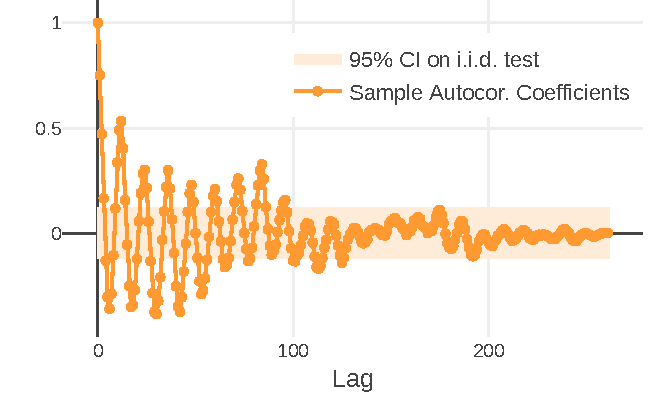
\includegraphics[scale=1]{Figures/plot_flocklab_autocorr.pdf}}

    \caption{Autocorrelation plot for the wireless link quality on FlockLab, based on the raw data collected by the testbed maintainers~\cite{jacob2019datasetLQE} (data from August 2019).
    \capt{The dataset contains one test every two hours. The first peak at lag 12 (\ie 24h) reveals the daily seasonal component. The data also show another at lag 84; which corresponds to one week. Indeed, there is less interference in the weekends than on weekdays: this creates a weekly seasonal component.}}
    \label{fig:flocklab_autocorr}
\end{figure}

\triscale assists the user in deciding on the time span for a series of runs, \ie when should the run be performed in a series. This is important to avoid biasing the evaluation results with time dependencies in the experimental conditions.
Indeed, it is common for real-world networks to exhibit periodic patterns.
For example, there may be a lot more cross-traffic (\ie interference) at specific times. In the statistics literature, these patterns are called \emph{seasonal components}.
Neglecting these may result in biased experiments leading to wrong conclusions, as illustrated in the case study below.

\fakepar{Case study: low-power wireless}
We run a simple evaluation of Glossy~\cite{ferrari2011Glossy}, a low-power wireless protocol based on synchronous transmissions~(\cref{sec:ST}). Glossy includes as parameter the number of retransmissions of a packet, called $N$. We investigate the impact of two values of $N$ on the reliability of Glossy, measured as the packet reception ratio (PRR). We define our KPI as the median with 95\% confidence level.
Refer to \cref{append:triscale_artifacts} for the complete case study.

We collect data using the FlockLab testbed~\cite{lim2013FlockLab}.
This testbed is located in an office building, where we expect more interference during daytime than nighttime.
Thus, we schedule a series of 24 runs randomly within one day.\\
  \inlineitem $N=1$ leads to a PRR of 88\%,\\
  \inlineitem $N=2$ leads to a PRR of 84\%.\\
In other words, it appears that doing two retransmissions (instead of one) reduces reliability.

The experiment leads to this (incorrect) conclusion because we have neglected a second seasonal component of the FlockLab testbed: there is a weekly time dependence, revealed by \Cref{fig:flocklab_autocorr}.
To account for this dependency, one must schedule runs with a span of at least one week. When comparing again the performance of Glossy but with tests spanning over a week\\
  \inlineitem $N=1$ leads to a PRR of 80\%,\\
  \inlineitem $N=2$ leads to a PRR of 88\%,\\
which better matches our knowledge about the performance of Glossy.

\fakepar{Conclusion}
This simple example illustrates that using a high confidence level is not enough to avoid drawing wrong conclusions due to the variability in the experimental conditions.
On a real network, short-term variations are unpredictable and (often) unavoidable. This is why it is important to perform multiple runs in a series: it increases the chances to do the experiment in the whole range of favorable to unfavorable conditions.

However, we illustrated that systematic patterns are also present. In other words, there are times where there is consistently more or less interference. Knowing about these dependencies is important to
  ensure fairness in the comparison between protocols, and
  enable reproducibility of the evaluations.
The series span must be long enough such that it does not matter when the series actually starts (\eg a weekend or a weekday)

\triscale integrates a network profiling function that analyzes link quality data (such as those available at~\cite{jacob2019datasetLQE}) and searches for seasonal components in the link quality data. This helps the experimenter detecting (sometimes unexpected) time dependencies, thus choosing a suitable time span for series of runs.


%-------------------------------------------------------------------------------
\subsection{Assessing Reproducibility}
\label{subsec:reproducibility}

Reproducibility refers to the ability of obtaining ``the same'' results when performing ``the same'' experiment.
In statistics, such property can be investigated using \textit{equivalence testing}~\cite{lakens2017Equivalence}, which checks whether the values of some parameter of interest (\eg the median) obtained for different samples are sufficiently close to be considered ``the same''.
Unfortunately, there is no general way to define ``sufficiently close''; one must define in advance a threshold for the equivalence test based on expertise.
Then, how to assess reproducibility of networking experiments? How to design a ``reproducibility test'' that fairly adapts to different networking contexts and different metrics?
After some failed attempts, we conclude that defining a generic threshold for equivalence testing in networking might not be possible. But it may not be necessary.

We argue that the most important is to confidently estimate the variability of the results, which \triscale computes with its variability score~(\cref{subsec:repeatability}).
This score \emph{quantifies reproducibility}: the larger the score, the less reproducible the results are.
Shall a binary cut between ``reproducible'' and ``not reproducible'' be desired, a threshold can be set based on the variability score; \eg ``Results are said reproducible when the variability score is less than 20\mbps.''.
Such a threshold can only be context-specific; thus, deciding on threshold values relates more to benchmarking and therefore goes beyond the scope of \triscale~(see discussion in \cref{sec:going_further}).
